\documentclass[a4paper, openany]{memoir}

\usepackage[utf8]{inputenc}
\usepackage[T1]{fontenc} 
\usepackage[english]{babel}
\usepackage{amsmath}
\usepackage{amssymb}

\usepackage{booktabs}
\usepackage{fancyhdr}
\usepackage{float}
\usepackage{indentfirst}
\usepackage{graphicx}
\usepackage[linewidth=1pt]{mdframed}
\usepackage{multicol}
\usepackage{fancyvrb}

\pagestyle{fancy}
\fancyhf{}
\fancyhead[LE]{\leftmark}
\fancyhead[RO]{\rightmark}
\fancyhead[RE, LO]{PSD}
\fancyfoot[LE, RO]{\thepage}
\fancyfoot[RE, LO]{Pete Gautam}

\renewcommand{\headrulewidth}{1.5pt}

\chapterstyle{thatcher}

\begin{document}

\chapter{Software Projects}
\section{Why software projects fail}
Software projects fail because it is difficult to develop software. In particular, it is difficult to develop:
\begin{itemize}
    \item a software of high quality,
    \item a software without defects, and
    \item a software which solves the customer's problem.
\end{itemize}

In the graph below, we can see how many projects failed over time.
\begin{figure}[H]
    \centering
    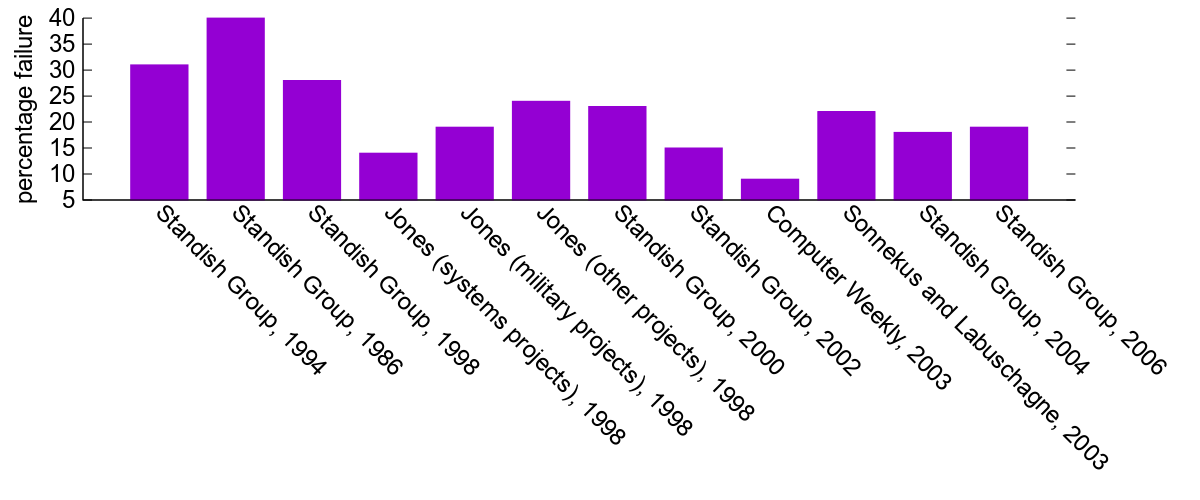
\includegraphics[scale=0.28]{src/1.1 NumberOfFailuresGraph.png}
    \caption{A graph which shows the percentage failure of software projects as described by different research papers.}
\end{figure}
\noindent From the graph, it is clear that a significant portion (between a third and a quarter) of software projects fail. We can see that in 1980s, about 40\% of projects failed according to Standish Group (1986). Moreover, even in 2006, about 20\% of the projects failed. 

There are many reasons why a software project fails, for example:
\begin{itemize}
    \item the software went over the budget,
    \item the software was over-scheduled, or
    \item the software did not meet the customer's requirements.
\end{itemize}
The graph below gives us an idea as to how many software projects failed for what reasons.
\begin{figure}[H]
    \centering
    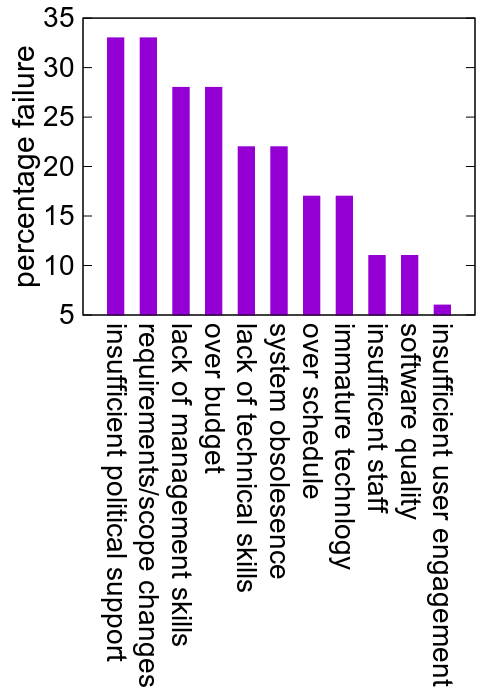
\includegraphics[scale=0.3]{src/1.2 WhyFailureGraph.png}
    \caption{A graph that shows how many software projects failed for what reasons (Emam and Koru (2008)).}
\end{figure}

\section{Case Studies}
In 1991, the London ambulance service wanted to automate their dispatch system. Earlier attempts to computerise the system had failed. The system went live on October 1992, and the system immediately had issues. In particular,
\begin{itemize}
    \item response to calls took longer than 11 hours;
    \item new calls wiped out previous calls that hadn't been responded (i.e. some people didn't receive an ambulance);
    \item vehicle location system didn't work about once every 53 times;
    \item 2 ambulances were sent to the same place at times.
\end{itemize}
The system was abandoned in 2 days. It cost £43 million, and it was originally estimated to cost £1.5 million. In general, the main issues with the software development were:
\begin{itemize}
    \item It was not realistic to fully automate the system with the available technology.
    \item There was a lack of consultation with the users.
    \item There was a pressure to deliver the system under tight budget and time schedule (both of which weren't realistic).
\end{itemize}

In 2007, the Scottish government wanted to automate scanning ballot papers since the electoral system had been changed. The software was developed in a reasonable timeline. It was split into multiple stakeholders. The system scanned ballot papers and then transferred the data into a database so that it could be processed manually. However, there were many issues when counting ballots:
\begin{itemize}
    \item It took longer than expected to scan ballots since the machines got jammed.
    \item About 140 000 ballots were rejected across Scotland, which was significantly higher than previous elections.
    \item The database became corrupted due to excess number of spoiled ballot papers.
\end{itemize}
Although there was acceptance testing with 10 000 ballots, these samples did not represent real user behaviour. Moreover, the number of samples were significantly lower than the actual number of ballots that were scanned during the election. This was the main issue with the software development.

\section{Issues in software development}
Brooks (1995) says that software development is difficult because it is intrinsically:
\begin{itemize}
    \item complex- there are many connected components within a software, which makes it difficult to think about a component by itself;
    \item intangible- a software has no physical form. Even though we can look at the source code, it is very different to the actual software- it is an abstraction;
    \item malleable- it is easy to change the behaviour of a software with few lines of code. This makes it very difficult to keep track of changes and their effects;
    \item large- a software can have millions of lines of code;
    \item evolutionary- a software is constantly changing, as we add more requirements to the software.
\end{itemize}

So, software projects fail because:
\begin{itemize}
    \item the system is built for the wrong reason;
    \item the system built is wrong (e.g. misunderstanding in the requirements); or
    \item the system is built in the wrong way (e.g. methods to ensure good quality of software were not followed).
\end{itemize}

\section{What is software engineering}
In order to develop software better, we can look at other disciplines of engineering. Moreover, we can define what we mean by software engineering. The following are few definitions of software engineering:
\begin{itemize}
    \item Sommerville (2010): software engineering is the principles, methods, techniques and tools for the specification, development, management and evolution of software systems;
    \item Bourque and Dupis (2005): software development is the application of a systematic, disciplined, quantifiable approach to the development, operation, and maintenance of software; that is, the application of engineering to software;
    \item Lethbridge and Laganiere (2005): the process of solving the customer's problems by the systematic development of large, high-quality software systems within cost, time and other constraints.
\end{itemize}
So, software engineering involves techniques to systematically build (and maintain) a software.

\section{Waterfall approach}
When software development was emerging, people looked to other engineering disciplines to establish the discipline of software development. One of the early approaches in software development was the waterfall approach. The stages of the waterfall approach are given below.
\begin{figure}[H]
    \centering
    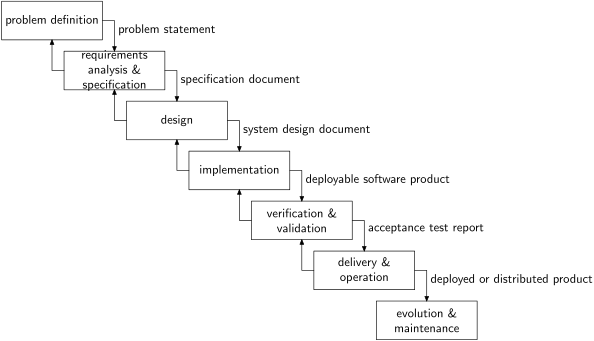
\includegraphics[scale=0.55]{src/1.3 Waterfall.png}
    \caption{The stages of the waterfall approach}
\end{figure}
\noindent The waterfall approach is composed of a series of stages, each of which followed from the previous one and led to the next one, like a waterfall.

This approach does not work because software has ultra-large scale complexity. In particular:
\begin{itemize}
    \item It is difficult for one software developer (or even a team) to manage all requirements and dependencies of a software.
    
    \item Software projects are unique- we cannot easily look at previous projects as a guide in future projects. In fact, if a project is similar to a previous one, we will just tweak it a bit instead of creating a new project. This makes it difficult to estimate the cost/time required for a given project.
    
    \item Software development is predominantly brownfield. Greenfield development (described by Hopkins and Jenkins (2008)) is when we do not have any pre-existing requirements/conditions that a software needs to obey. However, software development is quite the opposite- it is brownfield. For example, an organisation usually has a set of pre-existing software infrastructure (e.g. authentication services, email servers, APIs for data servers) that imposes constraints on the available design, features and implementation of the software.
    
    \item Software development is more about maintaining the infrastructure than the early stages of requirements gathering, designing and implementation. For instance, consider the following graph which highlights what proportion of a team's resources are spent on maintenance by different reports:
    \begin{figure}[H]
        \centering
        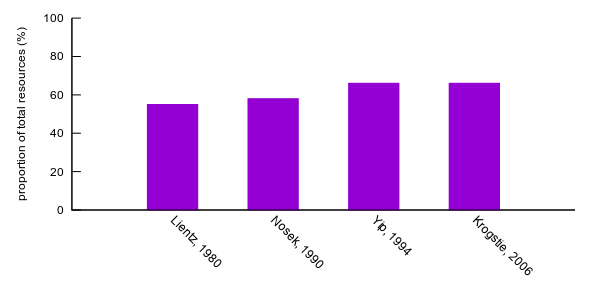
\includegraphics[scale=0.55]{src/1.4 InfrastructureMaintenance.png}
        \caption{What proportion of a team's resources are spent on maintenance, according to different reports}
    \end{figure}
    So, according to Krogstie (2006), about 60\% of total resources were allocated towards maintenance; everything else was only about 40\%.
\end{itemize}

In summary, the waterfall approach is misleading. It over-emphasises the early stages and under-emphasises the maintenance and evolution phases, which dominate a software project. The process is better thought of as an ongoing maintenance activity within which there are requirements, design, implementation and validation going on continually.

% TODO: Lc1, he talks about books and stuff at -2:00
Moreover, software projects are infrastructure maintenance- it involves implementation, with continual incremental improvement, measurement and review.

In conclusion, softwares are likely to fail due to the unique characteristics they have. Software engineering is aiming to reduce/manage these risks within software development. Instead of a one-off implementation, software engineering is more about maintenance of code.

\end{document}
